\chapter{Introduction and theory}
\label{chap:theory}

\section{The Standard Model of particle physics}
\subsection{Introduction}

The \SM of particle physics was put together during the second half of the 20$^{\text{th}}$ century. It has been an immensely successful theory, accurately describing all known processes in high energy physics encountered thus far~\cite{PDGBooklet}. The \SM is a \QFT, in particular a renormalisable gauge theory. In this model, the fundamental elements of matter, as well as the forces which govern their interaction, can be represented as relativistic quantum fields, the excitations of which are manifested as particles (see \Sec~\ref{sec:th:particlesandforces}). The \SM places all the forces except for gravity in the same framework, and unites the electromagnetic and weak forces into the electroweak force (see \Sec~\ref{sec:th:gauge}). The Higgs mechanism explains the manifest breaking of the underlying symmetry between these forces and leads to the prediction of an observable particle, the Higgs boson (see \Sec~\ref{sec:th:ewsb}). %All the particles postulated by the \SM have now been discovered, capped by the discovery of the Higgs boson in 2012.

%In order to do this, a mechanism ss required to permit the $W^{\pm}$ and $Z$ vector bosons to have mass while allowing the photon to remain masslesss. Such a theory was independently proposed by several theorists~\cite{BroutEnglert,Higgs1,Higgs2,Kibble1,Higgs3,Kibble2}, and is commonly referred to as the Higgs mechanism. In 1964, Higgs postulated that one outcome of this mechanism was that it should yield an observable particle, the Higgs boson~\cite{Higgs2}.



\subsection{Particles and Forces}
\label{sec:th:particlesandforces}
 In the \SM, matter is made up of \SpinHalf particles, called \emph{fermions}. Fermions come in two types: those wich interact exclusively via the eletroweak force, the \emph{leptons}, and those which can also interact via the strong nuclear force, the \emph{quarks}. The fermions can be arranged into three \emph{generations}, which are identical copies of each other, aside from the masses of the constituent particles. 
 %The first generation includes the electron (\Pe), the electron neutrino (\Pnue), the up quark (\Pup) and the down quark (\Pdown). The second generation includes the muon (\Pmu), the muon neutrino (\Pnum), the charm quark (\Pcharm) and the strange quark (\Pstrange). The third and final generation includes the tau (\Ptau), the tau neutrino (\Pnut), the truth or top quark (\Ptop) and the beauty or bottom quark (\Pbottom). 
Each of the particles mentioned in the table has a corresponding \emph{antiparticle}, with the same mass and opposite quantum numbers.
The \SM fermions and their properties are displayed in \Tab~\ref{tab:th:fermions}.

\begin{table}[h!]
 \resizebox{\textwidth}{!}{
\begin{tabular}{ |c | c l | c l | c l | }
\hline
type & \multicolumn{2}{|c}{ Generation I} & \multicolumn{2}{|c}{ Generation II} & \multicolumn{2}{|c|}{ Generation III} \\
\hline
  \multirow{4}{*}{leptons} & \Large{\Pe} & $m=0.511\MeV$ & \Large{\Pmu}  &   $m=105\MeV$ &   \Large{\Ptau}  &   $m=1777\MeV$  \\
                           &    electron &   $q=-1$      &  muon         & $q=-1$        &  tau      & $q=-1$   \\ \cline{2-7}
                           & \Large{\Pnue}       & $m\sim0\MeV$ & \Large{\Pnum}  &   $m\sim0\MeV$ &   \Large{\Pnut}  &   $m\sim0\MeV$  \\
                           &  electron neutrino  &   $q=0$      & muon neutrino  & $q=0$          &  tau neutrino    & $q=0$   \\
 \hline 
  
  \multirow{4}{*}{quarks} & \Large{\Pup} & $m=2.3\MeV$         & \Large{\Pcharm}  &   $m=1.275\GeV$  &   \Large{\Ptop}  &   $m=173\GeV$  \\
                          &      up      &   $q=+\frac{2}{3}$  & charm            & $q=+\frac{2}{3}$ & top or truth    & $q=+\frac{2}{3}$   \\ \cline{2-7}
                           & \Large{\Pdown} & $m=4.8\MeV$      & \Large{\Pstrange} &   $m=95\MeV$      &   \Large{\Pbottom}  &   $m=4.18\GeV$  \\
                           &        down    & $q=-\frac{1}{3}$ & strange           & $q=-\frac{1}{3}$  &  bottom or beauty   & $q=-\frac{1}{3}$   \\
 \hline 
  \end{tabular}
}
 \caption{The fundamental SM particles which constitute all matter in the universe are presented. The mass $m$ and electric charge $q$ are indicated for each particle \cite{PDGBooklet}.} 
\label{tab:th:fermions}
\end{table}

The matter particles interact via the fundamental forces. There are four known fundamental forces in the universe: the electromagnetic force, the weak nuclear force, the strong nuclear force and the gravitational force. The gravitational force is many orders of magnitude weaker than any of the other forces, and therefore has a negligible effect on the interactions of the \SM particles. Furthermore, no adequate quantum theory of gravity currently exists, therefore it cannot be easily included in the \SM. Therefore, the \SM deals only with the strong, weak and electromagnetic forces. In the \SM, the fundamental forces, are represented by the exchange of spin-1 \emph{mediator particles}, the \emph{vector bosons}. 
%The electromagnetic force is mediated by the photon (\Pphoton). The weak nuclear force is mediated by the Z-boson (\PZ) and the W-bosons (\PWplus and \PWminus). The strong nuclear force is mediated by the gluons (\Pgluon), of which there are eight, one for each possible linearly independent combination of colour charge (the strong force equivalent of electric charge).
The forces described by the \SM are listed in \Tab~\ref{tab:th:bosons}.

\begin{table}[h!]
 \resizebox{0.8\textwidth}{!}{
\begin{tabular}{ |c | c  | c  | c|  }
\hline
Force &  Indicative Strength & Mediator & Mass  \\
\hline
strong &  $1$ & gluons \Pgluon (8) & 0   \\
\hline
electromagnetic &  $10^{-3}$ & photon \Pphoton & 0   \\
\hline
 \multirow{2}{*}{weak} &  \multirow{2}{*}{$10^{-8}$} & W-boson \PWpm & 80.4 \GeV   \\
                       &                             & Z-boson \PZzero & 91.2 \GeV   \\
\hline
  \end{tabular}
}
 \caption{The three fundamental forces considered by the \SM are presented. For each force, the approximate strength relative to the strong force is shown, assuming two fundamental particles separated by a distance of $10^{-15}\m$. The mediator particle of each force is indicated along with its measured mass. \cite{Thomson:2013zua,PDGBooklet}}
\label{tab:th:bosons}
  \end{table}

The \Pphoton and \Pgluon are massless, in contrast to the \PWpm and \PZzero, which are massive. This difference is explained by the process of \emph{electroweak symmetry breaking} via the Brout-Englert-Higgs mechanism~\cite{Englert:1964et,Higgs:1964ia,Higgs:1964pj,Guralnik:1964eu,Higgs:1966ev,Kibble:1967sv} described in \Sec~\ref{sec:th:ewsb}. This mechanism introduces an additional field, which leads to an additional massive observable particle, the Higgs boson. This particle is predicted to be spin-$0$, and therefore it is referred to as a \emph{scalar boson}.

\subsection{Gauge groups of the SM Lagrangian}
\label{sec:th:gauge}

The Lagrangian $\mathcal{L}_{\text{QFT}}$ of a \QFT codifies the dynamics and interactions of its particles. %The equations of motion can be extracted using the \ELE. $\mathcal{L}_{\text{QFT}}$ 
It is constructed by considering the nature of the particles involved in the \QFT and imposing the symmetries which the theory ought to display. N\"other's Theorem~\cite{Noether} states that for every symmetry in a Lagrangian, there is an associated conservation law. For example, if a \QFT is invariant in time or space, this directly implies that the theory respects conservation of energy or momentum respectively. This simple example illustrates that imposing a symmetry in a Lagrangian places requirements on how the particles in the theory are allowed to propagate and interact. 

A gauge theory is a particular type of \QFT where local gauge transformations are a symmetry of the Lagrangian. Such gauge symmetries are of principal importance in particle physics, as they lead to the introduction of gauge fields, which generate the mediator particles. For this reason, the mediators of the forces are sometimes referred to as \emph{gauge bosons}. 
%The \SM is in fact a collection of gauge theories. 
Typically, a gauge transformation takes the form of shifting the quantum mechanical phase of all wavefunctions. It is reasonable to require such transformations to leave the dynamics of the theory intact, since the phase of a wavefunction is never manifest in any physical observable. Thus the Lagrangian of any realistic theory should be \emph{gauge invariant}, i.e. symmetric under phase transformation operations.  

\subsubsection{Quantum Electrodynamics}
\label{sec:th:qed}
A simple example of a gauge theory is \QED. 
%A single fermion is considered here (others can be trivially added). 
Fermions are described by the Dirac Lagrangian~\cite{griffiths2008introduction}:

\begin{equation}
\label{eq:th:dirac}
\mathcal{L}_{\textrm{fermion}} = i\overline{\psi} \gamma^{\alpha} \partial_{\alpha} \psi - m\overline{\psi}\psi,
\end{equation}

where $i$ is the imaginary unit, $\psi$ is a Dirac spinor and $\overline{\psi}$ is its adjoint, $m$ is the mass of the fermion, $\gamma^{\alpha}$ represents the Dirac gamma matrices and $\partial_{\alpha}$ is the 4-gradient. 
%Requiring \emph{global} gauge invariance means that we require that the Lagrangian is invariant under a global phase transformation
%\begin{equation}
%\label{eq:th:local_gauge_transform}
%\psi \rightarrow \psi'= \psi e^{i\theta},
%\end{equation}
%where $\theta$ is constant in time and space. This requirement is trivially satisfied by $\mathcal{L}_{\textrm{fermion}}$ :
%$$
%\mathcal{L}_{\textrm{fermion}} \rightarrow \mathcal{L}_{\textrm{fermion}}'=i\overline{\psi e^{i\theta}} \gamma^{\alpha} \partial_{\alpha} \psi e^{i\theta} - m\overline{\psi e^{i\theta}}\psi e^{i\theta}  =i \overline{\psi } e^{-i\theta} e^{i\theta}\gamma^{\alpha} \partial_{\alpha} \psi - m\overline{\psi} e^{-i\theta} e^{i\theta}\psi  = \mathcal{L}_{\textrm{fermion}},
%$$
%where it was possible to move $e^{i\theta}$ from the left to the right of the 4-gradient because $\theta$ is a constant. 

Requiring \emph{local gauge invariance} means that the Lagrangian should be  invariant under a phase transformation such as
$\psi \rightarrow \psi'= \psi e^{i\theta(\vec{x},t)}$, where $\theta(\vec{x},t)$ is some arbitrary differentiable function. Applying the transformation to \Eq~\ref{eq:th:dirac} gives:
\begin{equation}
\label{eq:th:dirac_lagrangian_not_invariant_local_gauge_transf}
\mathcal{L}_{\textrm{fermion}} \rightarrow \mathcal{L}_{\textrm{fermion}}'=  \mathcal{L}_{\textrm{fermion}} - \overline{\psi} \gamma^{\alpha} \psi (\partial_{\alpha} \theta(\vec{x},t)).
\end{equation}

Evidently $\mathcal{L}_{\textrm{fermion}}$ is not gauge invariant.
%even though this is a reasonable requirement for any theory which describes our universe. 
This is remedied by introducing an additional field $A_\alpha$. An extra term, $- g_{\textrm{EM}}\overline{\psi}\gamma^{\alpha}\psi A_{\alpha}$, is added to the Lagrangian to account for the interaction of the fermion with $A_\alpha$,
%$$
%\mathcal{L}_{\textrm{fermion+interaction}} = i\overline{\psi} \gamma^{\alpha} \partial_{\alpha} \psi - m\overline{\psi}\psi  - g_{\textrm{EM}}\overline{\psi}\gamma^{\alpha}\psi A_{\alpha},
%$$
where $g_{\textrm{EM}}$ is the strength of the interaction. Local gauge invariance is restored so long as $A_\alpha$ changes in the following way~\cite{griffiths2008introduction}: 

\begin{equation}
\label{eq:th:photon_gauge}
A_{\alpha} \rightarrow A_{\alpha} - \frac{1}{g_{\textrm{EM}}} \partial_{\alpha} \theta(\vec{x},t),
\end{equation}

%According to \Eq~\ref{eq:th:photon_gauge}, the interaction term transforms as:
%$$
%\mathcal{L}_{\textrm{interaction}} \rightarrow  \mathcal{L}_{\textrm{interaction}}' =  \mathcal{L}_{\textrm{interaction}}  + \overline{\psi} \gamma^{\alpha} \psi (\partial_{\alpha} \theta(\vec{x},t)),
%$$
%When applying the gauge transformation, the potential produces a $ + \overline{\psi} \gamma^{\alpha} \psi (\partial_{\alpha} \theta(\vec{x},t)) $ which exactly cancels out the additional term in \Eq~\ref{eq:th:dirac_lagrangian_not_invariant_local_gauge_transf}, thereby restoring gauge invariance.

The Lagrangian can also accomodate a term for $A_{\alpha}$ propagating freely through space. Since $A_{\alpha}$ is a 4-vector, it is described by the Proca equation for spin-1 bosons~\cite{griffiths2008introduction}:

\begin{equation}
\label{eq:th:proca}
\mathcal{L}_{\textrm{boson}} = -\frac{1}{16\pi} F^{\alpha\beta}F_{\alpha\beta} + \frac{1}{8\pi} m_{\textrm{boson}} A^{\alpha} A_{\alpha},
\end{equation}
where $F^{\alpha \beta} =(\partial^{\alpha} A^{\beta} - \partial^{\beta} A^{\alpha})$ and $m_{\textrm{boson}}$ is the mass of the spin-1 boson. 
\Eq~\ref{eq:th:proca} is locally gauge invariant so long as $m_{\textrm{boson}}=0$, i.e. the boson is required to be massless.

%The full Lagrangian for QED is therefore composed of a Lagrangian for: a free fermion,  a free spin-1 boson and a term for interactions between the boson and the fermion. 

%\begin{equation}
%\label{eq:th:QED_lagrangian}
%\mathcal{L}_{\textrm{QED}} = \underbrace{i\overline{\psi} \gamma^{\alpha} \partial_{\alpha} \psi - m\overline{\psi}\psi}_{\textrm{free fermion}}   \overbrace{-\frac{1}{16\pi} F^{\alpha\beta}F_{\alpha\beta}}^{\textrm{free spin-1 boson}}  \underbrace{- g_{\textrm{EM}}\overline{\psi}\gamma^{\alpha}\psi A_{\alpha}}_{\textrm{interaction term}}.
%\end{equation}
It is convenient to define the \emph{covariant derivative}, incorporating the interaction term:

\begin{equation}
\label{eq:th:covariant_derivative}
D_{\alpha} = \partial_{\alpha} + i g_{\textrm{EM}}A_{\alpha},
\end{equation}

so that $\mathcal{L}_{\textrm{QED}}$ can be written compactly as :

\begin{equation}
\label{eq:th:QED_lagrangian}
\mathcal{L}_{\textrm{QED}} = i\overline{\psi} \gamma^{\alpha} D_{\alpha} \psi - m\overline{\psi}\psi -\frac{1}{16\pi} F^{\alpha\beta}F_{\alpha\beta}.
\end{equation}

The full Lagrangian for \QED describes a free fermion, a free spin-1 boson and a term for interactions between the boson and the fermion. The boson is identified as the photon. The factor multiplying $g_{\textrm{EM}}$ is interpreted as the charge of the fermion.

The local gauge transformation is equivalent to applying a unitary $1\times1$ matrix to the wavefunction. The group of all such transformations is $U(1)$. It is a general principle that the number of degrees of freedom in the underlying symmetry group dictates the number of additional bosons needed to keep the theory locally gauge invariant~\cite{griffiths2008introduction}. 

\subsubsection{Quantum Chromodynamics}

The strategy described in \Sec~\ref{sec:th:qed} can be used to derive the Lagrangian for \QCD, which codifies the dynamics of the strong force~\cite{griffiths2008introduction}.  %~\cite{Han:1965pf,Fritzsch:1973pi}. 
The situation is more complicated because the underlying group is not $U(1)$ but $SU(3)$, which has eight degrees of freedom. This leads to eight massless gluons. In \QED, the interaction between the boson and the fermion is dictated by electric charge; the analogue for \QCD is \emph{colour charge}. However, colour charge cannot be represented by a single real number. Colours charges are instead linear combinations of \emph{red, antired, green, antigreen, blue, antiblue}. Each \SM quark has three identical copies with different colour charge. Another important difference is that $U(1)$ is abelian while $SU(3)$ is not. The consequence of this is that unlike the \QED photon, which carries no electric charge, the \QCD gluons carry colour charge. Gluons can therefore feel the strong force and self-interact. This fact leads \QCD to display unusual properties such as confinent of quarks and asymptotic freedom~\cite{PhysRevLett.30.1346,PhysRevLett.30.1343}. The gauge group for \QCD, $SU(3)_{\textrm{C}}$, is generally written with a subscript to indicate that it generates colour charge. 

\subsubsection{Electroweak unification}

%Although an equivalent of \QED exists for the weak force, \QFD, 
A major achievement of 20$^{\textrm{th}}$ century science was the unification of the electromagnetic and weak forces by Glashow, Weinberg and Salam~\cite{GlashowPartialSymmetries,WeinbergModelOfLeptons,SalamNobelSymposium}. %, thus superseding \QFD. 
Their \EWT considers the gauge group $SU(2)_{\textrm{L}} \times U(1)_{\textrm{Y}}$. The $SU(2)_{\textrm{L}}$ group has three degrees of freedom, so three gauge bosons and three types of charge are obtained from imposing local gauge invariance. The charges are called \emph{weak isospin}, and labelled $i_1, i_2, i_3$. The subscript in $SU(2)_{\textrm{L}}$ indicates that only left-handed particles carry nonzero weak isospin charge. The $U(1)_{\textrm{Y}}$ group behaves as in \QED, but generates \emph{weak hypercharge} $y$. The electric charge $q$ is related to weak isospin and weak hypercharge by the relation $q=y/2 + i_3$. The subscript in $U(1)_{\textrm{Y}}$ refers to the fact hypercharge is the generated charge.

Right- and left-handed fermions are considered separately in \EWT. It is helpful to think of the right-handed fermion spinors as \emph{singlets}, or column vectors of one spinor. For example, this is labelled $\Pe_{R}$, for the right-handed electron singlet.
The left-handed fermions come in \emph{doublets} (a column vector of two fermion spinors), e.g.:
$$
L_{\textrm{L}}=\binom{\Pnue}{\Pe}_{\textrm{L}},
$$
which is the left-handed lepton doublet containing the left-handed electron and electron neutrino. No right-handed neutrinos are included in this scheme. 

Imposing gauge invariance leads to the introduction of gauge fields: $W_{\alpha}^{1},W_{\alpha}^{2},W_{\alpha}^{3}$ and $B_{\alpha}$, for $SU(2)_{\textrm{L}}$ and $U(1)_{\textrm{Y}}$ respectively. The physical states observed in nature are mixtures of the underlying weak isospin and weak hypercharge gauge bosons:

\begin{equation}
\label{eq:th:electroweak_gauge_bosons}
\PWpm_{\alpha} = \sqrt{\frac{1}{2}}(W_{\alpha}^{1} \mp W_{\alpha}^{2}) ,\\
\PZzero_{\alpha} = \cos \theta_{W} W_{\alpha}^{3} - \sin \theta_{W} B_{\alpha} ,\\
A_{\alpha} = \sin \theta_{W} W_{\alpha}^{3} + \cos \theta_{W} B_{\alpha} ,
\end{equation}

where $\theta_{W}$ is the  is requiredWeinberg angle, which relates strengths of the electromagnetic ($g_{\textrm{EM}}$) and weak ($g_{\textrm{W}}$) forces via the relation $\tan \theta_{W} = g_{\textrm{W}} /g_{\textrm{EM}}$.

%\EWT successfully presents the electromagnetic and weak forces as manifestations of the same underlying electroweak force generated by $SU(2)_{\textrm{L}} \times U(1)_{\textrm{Y}}$. 
 Quarks are also accomodated in this framework. For example, for the first generation of quarks, two right-handed quark singlets $u_{R}$ and $d_{R}$ and one left-handed quark doublet $Q_{L}$ are introduced. The full \SM, incorporating the electroweak and strong forces, is descibed by the gauge group $SU(3)_{\textrm{C}} \times SU(2)_{\textrm{L}} \times U(1)_{\textrm{Y}}$.
 
 
An issue arises however, when considering masses of particles. 
%In \QED where the mass of a fermion is given simply by the term $ -m\overline{\psi}\psi$ in the Lagrangian, but the equivalent term, for example for the electron, must account for both the right-handed and left-handed components, which transform differently since one is a singlet and the other is part of a doublet. This breaks the gauge invariance of the fermion mass terms.
The left- and right-handed components of the fermions transform as doublets and singlets respectively, so the usual fermion mass term is no longer gauge invariant.
Furthermore, the gauge bosons should be massless to preserve the gauge symmetry. This is the case for the photon, but the \PWpm and \PZzero have experimentally measured masses of the order of 90\GeV~\cite{PDGBooklet}. A mechanism is needed to account for the masses of these particles. 

\subsection{Electroweak Symmetry Breaking and the Higgs Mechanism}
\label{sec:th:ewsb}

The process which allows the \PWpm and \PZzero to aquire a mass is \emph{electroweak symmetry breaking}. This occurs in the \SM via the Brout-Englert-Higgs mechanism~\cite{Englert:1964et,Higgs:1964ia,Higgs:1964pj,Guralnik:1964eu,Higgs:1966ev,Kibble:1967sv}. In this scheme, an additional complex scalar (spin-0) $SU(2)_{\mathrm{L}}$ doublet is introduced, which is denoted as $\phi$, and for which the Lagrangian is gauge invariant but the ground state is not. 
%Spin-0 boson singlets are described by solutions to the Klein-Gordon equation, which takes the following form in a Lagrangian:
%\begin{equation}
%\label{eq:th:klein_gordon_lagrangian}
%\mathcal{L}_{KG} = \frac{1}{2}(\partial_{\alpha} \Phi)^{*} (\partial^{\alpha} \Phi) - \frac{1}{2} (m_{\Phi})^{2} (\Phi^{*} \Phi)  ,
%\end{equation}
%where $m_{\Phi}$ is the mass of the sping-0 scalar boson $\Phi$.
The Lagrangian which is chosen for $\phi$ is of the form:

\begin{equation}
\label{eq:th:higgs_lagrangian}
\mathcal{L}_{\phi} = \frac{1}{2}(D_{\alpha} \phi)^{*} (D^{\alpha} \phi) + \frac{1}{2} \mu^{2} (\phi^{*} \phi) - \frac{1}{4} \lambda^{2} (\phi^{*} \phi) ^{2} ,
\end{equation}

where $\mu$ and $\lambda$ are constants. The covariant derivative $D_{\alpha}$ defined in \Eq~\ref{eq:th:covariant_derivative} has been used here to ensure gauge invariance. In this case, $D^{\alpha}$ also accounts for the interactions with the $\PWpm, \PZzero$ and gluons in addition to the photon.
The first term of the Lagrangian corresponds to the kinetic part, while the second and third correspond to a potential. %Comparing to \Eq~\ref{eq:th:klein_gordon_lagrangian}, 
The term $ \frac{1}{2} \mu^{2} (\phi^{*} \phi)$ resembles a mass term, but it is not: the sign needs to be negative. If $\mu^{2}<0$, the potential has a non-zero \VEV, and the ground state is represented by a circle of minima. In order to re-write the Lagrangian in terms of physical particles, an expansion around one of the minima is required. Since they are all equivalent, an arbitrary minimum is chosen:

\begin{equation}
\label{eq:th:higgs_vev}
\phi_{0} = \VEV = \frac{1}{\sqrt{2}} \binom{0}{v} ,
\end{equation}
where $v=\sqrt{- \mu^{2} / \lambda}$. At this stage, any of the minima lying upon the circle of ground states could have been chosen, but in order to find the physical states in the Lagrangian, a particular choice had to be made. This step breaks the manifest symmetry in the physical states while preserving it in the Lagrangian. 

To obtain the physical states from this Lagrangian, a small perturbation field, $H$, around the \VEV is introduced: 

\begin{equation}
\label{eq:th:higgs_vev_perturbation}
\phi = \frac{1}{\sqrt{2}} \binom{0}{v+H} ,
\end{equation}
which can be substituted back into the original Lagrangian in \Eq~\ref{eq:th:higgs_lagrangian}. Expanding out the implicit interactions with the gauge bosons from the covariant derivative, the equation becomes:

\begin{equation}
\begin{split}
%\mathcal{L}_{\phi} = \frac{1}{2} (\partial_{\alpha} H) (\partial^{\alpha} H) - \frac{1}{2} \mu^{2} H^2 + \frac{v^2}{8}( g_{\textrm{W}} \PWp_{\alpha}\PWp^{\alpha} + g_{\textrm{W}} \PWm_{\alpha}\PWm^{\alpha} + (g^2_{\textrm{W}}+g^2_{\textrm{EM}})  \PZzero_{\alpha}\PZzero^{\alpha}) + ...,
  \mathcal{L}_{\phi}  =  \frac{1}{2} & (\partial_{\alpha} H) (\partial^{\alpha} H) - \frac{1}{2} \mu^{2} H^2 \\
&  + \frac{v^2}{8}( g_{\textrm{W}} \PWp_{\alpha}\PWp^{\alpha} + g_{\textrm{W}} \PWm_{\alpha}\PWm^{\alpha} + (g^2_{\textrm{W}}+g^2_{\textrm{EM}}) \PZzero_{\alpha}\PZzero^{\alpha}) + ...
\end{split}
\end{equation}
\label{eq:th:higgs_lagrangian}
where terms which do not correspond to mass-like terms have been omitted.
%Now that the Lagrangian has ben re-written after expansion around a valid minimum, the physical states can be identified.
%it with the Klein-Gordon equation% in \Eq~\ref{eq:th:klein_gordon_lagrangian}. 
The first two terms can be identified as the Klein-Gordon equation for a massive scalar boson of mass $\sqrt{2}\mu$: this is the Higgs boson. The other terms represent the great success of the Brout-Englert-Higgs mechanism: the \PWpm and \PZzero bosons have acquired masses. The absense of equivalent terms for the photon and gluons means that they do not aquire masses, which is in accordance with experimental expectations.

%Adding $\mathcal{L}_{\phi}$ to the \SM Lagrangians for \EWT and \QCD maintains local gauge invariance, but allows the weak force mediators to acquire mass. 
Furthermore, it is possible to add additional gauge invariant terms involving the scalar field. These are known as the Yukawa terms. For example, in the case of the first generation leptons:

\begin{equation}
\label{eq:th:yukawa_coupling}
\begin{split}
  \mathcal{L}_{\textrm{Yukawa}} &= \kappa_{e} (\overline{L} \phi  e_{R} + \overline{e_{R}} \phi^{\dagger} L )\\
                       &=  \kappa_{e} v (\overline{e_{L}} e_{R} + \overline{e_{R}} e_{L} ) +  \kappa_{e}   (\overline{e_{L}} H e_{R} + \overline{e_{R}} H e_{L} ),
\end{split}
\end{equation}
where $\kappa_{e}$ is a real constant. The first term is as a mass term for the electron and the second is the interaction term between the electron and the Higgs boson. By construction, the strength of the interaction is directly proportional to the mass of the particle which is considered. Furthermore, the neutrino does not acquire any mass via this mechanism. The scheme described above does not prescribe the masses however: these are free parameters in the theory are must be specified from experimental measurements.

To summarise, the Brout-Englert-Higgs mechanism adds a gauge-invariant terms to the \SM Lagrangian which permits the $\PWpm$ and $\PZzero$ bosons and the fermions to acquire a mass while leaving the gluons and the photon massless. The outcome is one additional particle, the Higgs boson, which is a massive spin-0 particle, the Higgs boson. 

 
\section{Higgs boson phenomenology}
\subsection{History of Higgs boson searches}

Since the Higgs boson was postulated in the 1960s, there have been many experimental efforts to try to observe it. Theoretical considerations precluded large Higgs boson masses above the order of 1\TeV~\cite{Heller:1993yv}. Experiments conducted before the start of \LEP operation excluded a Higgs boson of mass below the order of 10\GeV~\ref{Wu:2014vva}. Direct searches at \LEP and the Tevatron excluded a Higgs boson mass below 114\GeV~\cite{Barate:2003sz,TEVNPH:2012ab}, and precision measurements of the electroweak parameters suggested that the Higgs boson mass should be below 200\GeV~\cite{Renton:2004wd}. The search for the Higgs boson prompted the construction of the \LHC at \CERN, and two multi-purpose detectors, \ATLAS and \CMS, were designed with the Higgs observation as one of their main physics goals. In 2012, the two experiments jointly announced the observation of a Higgs-like particle of mass $\sim$125 GeV, ending a 50-year interval between postulation and discovery~\cite{CMSHDisc,ATLASHDisc}.

\subsection{Higgs boson production at the LHC}

According to \SM (see \Eq~\ref{eq:th:yukawa_coupling}), the Higgs boson interacts with particles proportional to their masses. Five production modes can lead to the production of a Higgs boson in \pp collisions at the \LHC. The Feynman diagrams for these processes can be seen in \Fig~\ref{fig:theory:higgsproduction}. The most likely production mode for  $\mH=125.09\GeV$ is \ggH via a loop of top quarks, which has a cross section of approximately 49\pb at 13\TeV. The other production modes are \VBF at 3.8\pb, \WH at 1.4\pb, \ZH at 0.9\pb , and \ttH at 0.5\pb~\cite{LHCHXSWGRY4}. The \WH and \ZH modes are often considered together are referred to as \VH.

  \begin{figure}[h!]

  \centering
  \subfloat[]{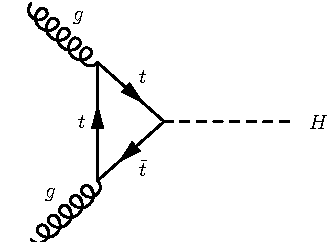
\includegraphics[width=0.24\textwidth]{theoryFigures/ggH.pdf}}
  \subfloat[]{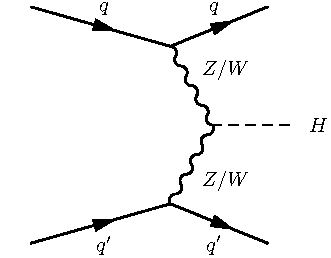
\includegraphics[width=0.24\textwidth]{theoryFigures/vbf.pdf}}
  \subfloat[]{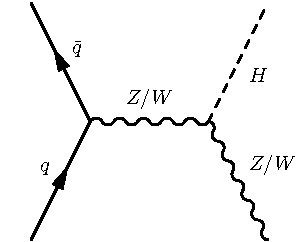
\includegraphics[width=0.24\textwidth]{theoryFigures/wzH.pdf}}
  \subfloat[]{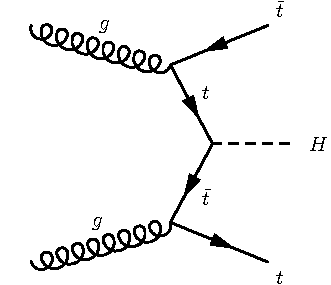
\includegraphics[width=0.24\textwidth]{theoryFigures/ttH.pdf}}
  \caption{Higgs production modes at the LHC: (a) gluon-gluon fusion, via a loop of top quarks, (b) vector boson fusion, with associated quark production, (c) associated vector boson production with either the \PZzero or \PW boson and (d) top quark fusion with associated top quark production. }
  \label{fig:theory:higgsproduction}
  \end{figure}

\subsection{Higgs boson decays}


The \SM Higgs boson can decay either directly to pairs of particles, or via virtual loops.
In direct decays to pairs of particles, the  branching ratios are proportional to the mass of the decay product. The most likely direct decay modes to massive particles for a \SM Higgs boson with $\mH=125.09\GeV$ are $\PH \rightarrow \Pbottom \Pbottom$ (58.2\%), $\PH \rightarrow \PW \PW^{*}$ (21.4\%), $\PH \rightarrow \Ptau \Ptau$ (6.3\%), $\PH \rightarrow \PZ \PZ^{*}$ (2.6\%)~\cite{LHCHXSWGRY4}. The production of a pair of $t$ quarks is not kinematically allowed. The Higgs coupling to electrons, muons, neutrinos, up quarks, down quarks and strange quarks is very small due to the mass of the decay products.
In addition, Higgs boson decays can occur via a loop of virtual massive particles. In this way, the Higgs boson can decay to a pair gluons (8.2\%), to a pair of photons (0.23\%) or to $\PZzero\gamma$ (0.02\%)~\cite{LHCHXSWGRY4}. 

Despite the low branching fraction, the decay \Hgg played a key role in the discovery of the Higgs boson. This is because it has a very clean signature of two highly energetic photons in the detector, with an irreducible but controllable \SM background. This is in contrast with some of the other more frequent decay modes, where difficulties in reconstructing the decay products or excessive noise from the \LHC \pp collisions drastically reduce the experimental sensitivity. The Feynman diagram for the \Hgg decay can be seen in \Fig.~\ref{fig:theory:higgstogammagamma}. 

\begin{figure}[h!]
    \begin{fmfgraph*}(100,100)
      \fmfright{o0,o2,ox,o3,o5}
      \fmfleft{i0,i3,i1,i4,i6}
      \fmf{phantom,tension=4/3}{o2,v1,i3}
      \fmf{phantom,tension=4/3}{o3,v2,i4}
      \fmffreeze
      \fmf{photon,tension=4/3}{o2,v1}
      \fmf{photon,tension=4/3}{o3,v2}
      \fmf{fermion,tension=0,label=$t$}{v1,v2}
      \fmf{fermion,tension=2/3,label=$\bar{t}$}{v2,v3}
      \fmf{fermion,tension=2/3,label=$t$,label.side=right}{v3,v1}
      \fmf{dashes}{v3,i1}
      \fmflabel{$\gamma$}{o2}
      \fmflabel{$\gamma$}{o3}
      \fmflabel{$H$}{i1}
  \end{fmfgraph*}  
  \caption{A Higgs boson decaying to a pair of photon via a loop of top quarks. It is also possible for the photons to be produced via  a loop of \PW bosons, although this far less likely.}
    \label{fig:theory:higgstogammagamma}
    \end{figure}

%\subsection{Higgs boson measurement motivation}
 
%Although the \SM has been very successful as a theory, it falls short of being a “``theory of everything'', and is clearly incomplete. For instance, it does not accommodate mass terms for neutrinos, which are required to explain the origin of neutrino oscillations observed in many experiments~\cite{SuperK,SNO,DayaBay}. Furthermore, it does not contain a viable candidate for dark matter, which may be needed to explain the mass deficit of the universe~\cite{DM}. Other issues such as the hierarchy problem~\cite{Hierarchy} and the origin of matter-antimatter asymmetry~\cite{Asymmetry} also persist. Clearly, the \SM is incomplete or approximate, and many efforts in modern high energy physics are being made to discover \BSM physics. Detailed studies of the properties of the newly-discovered Higgs boson could provide valuable insight into the nature or indeed existence of \BSM physics.
